\chapter{Umsetzung}
\label{chap:umsetzung}
    Im Rahmen einer prototypischen Implementierung wurde das im Konzept (siehe Kapitel \ref{chap:konzept}) geplante System
    umgesetzt. Gegenstand dieses Kapitels wird es sein, Aspekte der Umsetzung widerzuspiegeln und konkret die Umsetzung eines  
    Anwendungsfalls darzulegen. Zusätzlich wird die Auswahl des dafür genutzten Frameworks aufgegriffen. 

\section{Auswahl des Frameworks}
\label{sec:frameworkauswahl}
    Im Bereich der Java-Entwicklung gibt es mittlerweile viele Möglichkeiten, um Applikationen, Anwendungen und Frameworks 
    zu entwickeln, die unterschiedliche Präferenzen und Einsatzmöglichkeiten bieten. Dadurch sind, auf den Einsatzbereich bezogen, 
    Vor- und Nachteile im Vergleich ähnlicher Systeme nicht auszuschließen. Eine kleine Auswahl an Systemen wurde getestet und auf deren 
    Brauchbarkeit analysiert und evaluiert. Für diese Evaluation wurden Kriterien ausgearbeitet, mit der die Auswahl des Frameworks 
    eingeschränkt und nach Möglichkeit das passende ergeben soll. Die Kriterien sind nach ihrer Relevanz aufgelistet: 
    \begin{enumerate}
        \item Freiheiten bei der Nutzung (Anwendung und Gewährleistung von Entwurfsmustern).
        \item Nutzung und Bereitstellung von Bibliotheken (Libraries).
        \item Bereitstellung einer Plattform (Full Stack).
        \item Aktive Community und stetige Weiterentwicklung des Systems.
        \item Nutzung des Frameworks in bereits bestehenden Projekten im Bereich Smart Home.
        \item Open Source-Projekt, um Flexibilität und weitestgehende Unabhängigkeit zu gewährleisten.
        \item Ausschluss von Frameworks, die ausschließlich für die Web-Entwicklung gedacht sind.
    \end{enumerate}  
    Aufgrund der Vielzahl an Frameworks war es im Rahmen dieser Arbeit nicht möglich, alle vorhandenen und in Betracht 
    gezogenen Systeme detailliert aufzuführen. Lediglich die engere Auswahl wird aufgegriffen. 
    Nach ausführlicher Recherche und unter Berücksichtigung von Frameworks, wie bspw. Grails, Quarkus, Blade, und Play, wurden 
    schließlich genau zwei Systeme genauer betrachtet, die die vorangestellten Kriterien in Gänze erfüllen. Viele in Betracht gezogenen Frameworks 
    finden überwiegend in der Web-Entwicklung Anwendung, bzw. basieren auf dem Spring Framework. Durch diese Erkenntnis wurden 
    viele Systeme nicht weiter berücksichtigt. Die beiden Kernsysteme, die ihren Einsatz und ihre Möglichkeiten rechtfertigen
    werden in den folgenden Abschnitten kurz erläutert.

    \subsection{OSGi}
    \label{subsec:osgiFramework}
        Das \ac{OSGI} Framework der \acs{OSGI}\footnote{Ursprung der OSGi Plattform. \url{https://www.osgi.org/about/} Abgerufen am 19.06.2022} 
        Alliance, welches in der openHAB Software eingesetzt wird, klassifiziert eine dynamische Softwareplattform, mit der die Modularisierung 
        und Verwaltung von Applikationen und den dazugehörigen Diensten mittels Komponentenmodell realisiert werden kann \cite{funke2009}. Bekannte 
        Produkte, die auf der \acs{OSGI} Plattform laufen, sind neben openHAB unter anderem die Entwicklungsumgebung Eclipse der Eclipse 
        Foundation, Produkte und Softwarelösungen von IBM, Oracle, Adobe und weitere. 
        \\
        Nennenswerte Eigenschaften und Vorteile der Software sind die Modularisierung und Versionierung, das zur Laufzeit organisierte 
        Abhängigkeitsmanagement, das Fernmanagement des laufenden Systems über sogenannte Management Agents und die Nutzung des 
        Serviceorientierten Programmiermodells, \ac{SOA}\footnote{Erläuterung des SOA Modells. \url{https://www.ibm.com/cloud/learn/soa} Abgerufen am 20.06.2022}. 
        An dieser Stelle wird das Framework nicht technisch vertieft. Die Funktionsweise und die technisch 
        fundierte Erläuterung kann dem Buch \cite{osgibuch}, sowie der Dokumentation \cite{osgipraesentation} eines ausgearbeiteten Workshops entnommen werden. 
        Nachteile der Plattform sind zum einen der weniger breite Einsatz des Frameworks und zum anderen die kleine Community. 
        Ebenso findet eine Weiterentwicklung der Plattform nur mäßig statt. Dies hat zur Folge, dass die Erweiterung, bzw. die Entwicklung des darauf 
        aufbauenden Systems träge vonstattengeht. 
        %Wieso Spring Boot und nicht OSGi?
        %Wieso Java und nicht Python oder andere?

    \subsection{Spring}
    \label{subsec:springBootFramework}
    Spring\footnote{Open-Source-Framework Spring. \url{https://spring.io} Abgerufen am 02.07.2022} ist ein Open-Source-Framework, welches auf der Java-Plattform aufbaut. 
    Das Ziel von Spring selbst ist die Vereinfachung und Förderung von Programmierpraktiken in der Java- und Java EE Entwicklung. Mit einem breiten Spektrum an 
    Funktionalitäten bietet das Framework eine ganzheitliche Lösung zur Entwicklung von Applikationen, Anwendungen und Frameworks. Im Vordergrund dabei steht immer die 
    Entkopplung von Applikationskomponenten. Das Spring Framework wurde im März 2004 offiziell Freigegeben und wird seitdem stetig weiterentwickelt. 
    Initiator des Frameworks ist der Author und Softwareentwickler Rod Johnson. Das Framework, welches in dem Buch des Experten Rod Johnson erläutert wird, basiert auf 
    den folgenden Prinzipien \cite{johnson2004expert}: 
    \\
    \linebreak
    Dependency Injection ist ein sehr bekanntes Entwurfsmuster. Dabei werden die Abhängigkeiten eines Objektes zur Laufzeit reglementiert. Unter 
    Verwendung des Frameworks werden den Objekten die benötigten Objekte und Ressourcen zugewiesen. Dadurch müssen diese nicht selbst gesucht werden. 
    \\
    \linebreak
    Ein weiterer Punkt ist die aspektorientierte Programmierung, durch die der Entwickler technische Aspekte voneinander isolieren und den eigentlichen Programmcode 
    von Transaktionen oder anderen Faktoren freizuhalten. 
    \\
    \linebreak
    Das dritte Prinzip ist das Bereitstellen von Vorlagen zur Vereinfachung der Nutzung von Schnittstellen, sog. \acs{API}s. Dadurch wird ein POJO-basiertes Modell 
    möglich. Unter POJO, \textit{Plain Old Java Object}, ist ein ganz normales Objekt in Java zu verstehen. 
    \\
    \linebreak
    Zusammenfassend sind beide Frameworks dazu geeignet, um das Konzept der Steuerzentrale unterstützend zu realisieren. 
    Ein direkter Vergleich zwischen den Frameworks kann nicht gezogen werden, da die Funktionalitäten, bzw. die aus der Nutzung 
    profitablen Eigenschaften nicht vergleichbar sind. Während sich Spring auf die Unterstützung zur Erstellung von Applikationen konzentriert, 
    legt \acs{OSGI} den Mehrwert auf die Modularisierung durch Kontainerisierung. Durchaus ist eine Kombination aus beiden 
    Frameworks möglich, um Vorteile beider zu vereinen. Fundamental bietet Spring jedoch weitaus mehr Möglichkeiten und Unterstützungen 
    zur Entwicklung von Applikationen und Frameworks, weshalb es im Rahmen dieser Arbeit eingesetzt wird. Mit Spring Boot, welches auf Spring 
    aufbaut können auch \acl{MVC} Web-Architekturen und \acs{REST} \acs{API}s implementiert werden. So kann mit dieser Entscheidung 
    ein Vollumfängliches System erstellt werden. Unter zusätzlicher Verwendung von \acs{OSGI} wäre eine weiter Modularisierung und Kontainerisierung möglich. Dies 
    ist auch durch Spring mit Hilfe von Microservices in einer anderen Form realisierbar. 
    \\
    An der Stelle wird im Rahmen dieser Arbeit das Thema von Microservices und Kontainerisierung nicht weiter konkretisiert.
    \\
    \linebreak
    Die Entscheidung viel auf Spring, da dieses ein modernes und etabliertes Framework darstellt und die 
    Community erheblich größer ist, als die des \acs{OSGI} Frameworks. Hinzukommt, die Schaffung eines alternativen Ansatzes zu openHAB, da dieses System bereits 
    auf \acs{OSGI} aufbaut. 
    Dennoch unterscheidet sich die Steuerzentrale in den Funktionalitäten und Angeboten immens im Vergleich zu openHAB. Das System bietet weitaus mehr 
    Funktionalitäten, Erweiterungen und Ausprägungen. Lediglich kann zum Vergleich die Definition von Regeln herangezogen werden. 

\section{Implementierung}
\label{sec:implementation}
    Hierbei wird konkret die Implementierung des Frameworks aufgegriffen und beschrieben, wie Konzeptentscheidungen im Code umgesetzt wurden. 
    Auch werden wichtige Anhaltspunkte ergänzt, die in der Tiefe nicht aus dem Konzept hervorgehen, da dort lediglich die Idee und die allgemein gehaltene 
    Vorstellung skizziert wurde. 

\subsection{Generische Programmierung} % Typisierung
% Erledigt! -> WICHTIG!!!: Verwendung der Typisierung, um dem Anwender die Möglichkeit der offenen Gestaltung des Zustandobjektes zu gewährleisten.
Eine entscheidende Überlegung der Umsetzung in Richtung des Zustandsraumes ist die Verwendung der generischen Programmierung. 
\\
Mit dem Hintergrund, dass der Entwickler die volle Entscheidungsmacht über die Implementierung der 
Regeln, des Zustandsraumes und den dafür notwendigen Bedingungen beibehält, ist die Überlegung  
notwendig, wie mit einem Objekt gearbeitet werden kann, ohne dass es vorher bekannt ist. 
\\
\linebreak
Hierfür wird auf das Konzept der generischen Programmierung, sog. \textit{Generics}, gesetzt. Ein Synonym 
des Begriffs ist der parametrisierte Typ. Mit der Nutzung von Generics ist ein syntaktisches Mittel 
gegeben, mit dem Klassen und Methoden mit Typen parametrisiert werden können. Diese Typ-Variablen sind zum 
Zeitpunkt der Implementierung unbekannt und können beliebig definiert werden. Erst zur Laufzeit des Systems 
wird die Typ-Variable durch einen oder ggf. auch mehrere Typen ersetzt. Somit ist zur Laufzeit das 
Objekt, dessen Struktur, Methoden und Funktionen bekannt. Bei der Verwendung von generischen Typen gibt es 
Varianzfälle, die unterschiedliche Auswirkungen aufzeigen. Der für das Konzept relevante Fall ist der des 
einfachen Typ-Parameters. Weitere Varianzfälle werden in dieser Ausarbeitung nicht erläutert. 
\\
\linebreak
Ein konkretes Anwendungsbeispiel, wie es 
auch im Rahmen dieser Arbeit verwendet wird, sieht wie folgt aus:
\\
Das Framework arbeitet mit dem generischen Typ \textit{E}. Der Anwender soll nach der Implementierung der Klasse des Zustandsraumes das 
jeweilige Objekt dem Framework übergeben. So ist zur Laufzeit das konkrete Objekt bekannt. Zur Veranschaulichung dient folgendes Code-Beispiel:
\begin{lstlisting}[language=Java, frame=lines, xleftmargin=\parindent, style=algoBericht, label={code:generics}, captionpos=b, caption={Zustandsobjekt als Typ-Variable}]
public class LogicHub<E> {
    private E state;
    ...
    public E getState() {
        return this.state();
    }
    ...
}

public class Application {
    private final LogicHub<InnovationLab> logicHub;

    public static void main(String[] args) {
        logicHub = LogicHub.getInstance();
        logicHub.getState(); // -> returns the state object 
                             // and it's values.
        ...
    }
}
\end{lstlisting}
Mit den Java Generics ist eine leistungsstarke Ergänzung der Java-Sprache gegeben, da es die Arbeit des Programmierers einfacher und 
weniger Fehleranfällig macht. Zusätzlich wird durch die Generics die Typkorrektheit zur Kompilierzeit erzwungen und ermöglicht 
die Implementierung generischer Algorithmen, ohne für Anwendungen einen zusätzlichen Overhead zu verursachen. 
\\
Mit der Option des generischen Typs kann das Framework universell definiert und der Zustandsraum vom Anwender individuell implementiert werden.
\\
\linebreak
Durch die Verwendung der Java Generics wird der konzeptionelle Schnitt zwischen Framework und Anwender-Interaktionen deutlicher.
%Die Darstellung des Zustandsobjektes wird als bereits bestehendes vorausgesetzt, um die folgenden Diagramme vollständig und sinngemäß wiederzugeben. 
%Diese beschreiben jedoch zu keinem Zeitpunkt eine konkrete Struktur des Zustandsobjektes. 
%\\
%\linebreak
%Im weiteren Verlauf wird der Aufbau des Frameworks erläutert, sowie die detaillierte Beschreibung der einzelnen Schichten und deren Funktionalität. 

\subsection{Parallelisierung}
    Bereits im Konzept wurde der Terminus der Parallelisierung und der Asynchronität aufgegriffen. Für das Auslösen einer Regel, wird der gesamte Prozess der 
    Bedingungsprüfung und der anschließenden Ausführung in einen \textit{Thread} ausgelagert, der durch einen \textit{ThreadPoolExecutor}\footnote{Spezifikation des Thread-Pools. \url{https://docs.oracle.com/javase/7/docs/api/java/util/concurrent/ThreadPoolExecutor.html} Besucht am 27.07.2022} im java Code angestoßen wird. 
    Durch das Auslagern des konkreten Prozesses in einen eigenen \textit{Thread} können mehrere Regeln gleichzeitig ausgeführt werden, sofern die Bedingungsprüfung zutrifft und die 
    Regel ausgeführt wird. 
    In folge der Entscheidung, dass nach jeder Zustandsänderung immer alle Regeln durchlaufen werden, wäre eine sequenzielle Ausführung der Regeln sehr ineffektiv und langsam. Dadurch 
    würde sich das Durchführen von Regeln verzögern, bspw. wenn ein Licht eingeschaltet werden würde, davor allerdings noch zwei Regeln abgearbeitet werden müssten, die jeweils eine 
    Minute beanspruchen, würde sich das Licht erst nach zwei Minuten einschalten. Durch die Auslagerung des Regelmanagements in jeweils eigene \textit{Threads} entfällt die sequenzielle 
    Abarbeitung, da diese asynchron durchgeführt wird. Durch die Parallelisierung der Regelprozesse können gleichzeitig weitere Zustandsänderungen entstehen, die anschließend 
    wieder zusammengeführt werden und darauf gegebenenfalls weitere Regeln ausgeführt werden. An der Stelle der Zustandsänderung selbst greift der 
    Lock-Mechanismus, der durch einen \textit{ReentrantLock}\footnote{Spezifikation des Locks. \url{https://docs.oracle.com/javase/7/docs/api/java/util/concurrent/locks/ReentrantLock.html} Besucht am 27.07.2022} realisiert ist. Dadurch wird sichergestellt, dass der Zustandsraum, der die aktuell geltenden Zustände wiedergibt, immer nur einen Änderungsvorgang durchführt. 

\subsection{Reflection} 
    Mit der Reflection\footnote{Java Reflection. \url{https://www.oracle.com/technical-resources/articles/java/javareflection.html} Besucht am 27.07.2022} 
    (Reflexion, Spiegelung) ist eine Funktion der Programmiersprache Java gegeben, die es ermöglicht, Laufzeitattribute von Klassen, Schnittstellen, Feldern 
    und Methoden zu überprüfen und zu ändern. Diese Funktion erweist sich als besonders praktisch, wenn die Namen der Attribute zur Kompilierzeit nicht bekannt sind. 
    %dass ein ausgeführtes Programm bzw. ein erzeugtes Objekt sich während der Laufzeit selbst beobachtet und interne Eigenschaften darüber manipuliert werden können.
    Darüber hinaus können neue Objekte instanziiert, Methoden aufgerufen und Feldwerte mithilfe von Reflexion abgerufen oder festgelegt werden. 
    \\
    \linebreak
    Eingesetzt wird die Reflexion in der Transformation, die der Entwickler definiert, um aus eingehenden Events und Nachrichten Zustandsänderungen zu erzeugen. Konkret wird in der 
    Transformation der Name des Feldes mitgegeben, der vom Entwickler bei der Definition des Zustandsobjektes vergeben wurde. Somit kann immer auf das Feld und dessen Wert zurückgegriffen werden und bei Bedarf durch eine eingehende Nachricht, bzw. durch eine Zustandsänderung innerhalb einer Regel überprüft und geändert werden. Die Struktur der 
    Transformation wird in folgendem abschnitt greifbar aufgezeigt.

\subsection{Transformation}
    Die Transformation stellt die Schnittstelle zwischen den externen Auslösern, bspw. \acs{MQTT}, und der Kommunikationsschicht dar. 
    Die über das Kommunikationsprotokoll gelieferten Daten werden der \textit{transform}-Methode übergeben, sodass die eigentliche 
    Transformation stattfinden kann. %Die Struktur der Transformation wird vorab erläutert, damit die anschließende Erläuterung 
    %übertragbar ist. 
    \\
    \linebreak
    Im Rahmen der Arbeit wurden zwei Lösungswege erarbeitet, die jeweils dem Entwickler ermöglichen, eine Transformation zu definieren. Diese werden beide 
    erläutert und anschließend gegenübergestellt. Das dabei verfolgte Ziel, ist dem Anwender einen möglichst komfortablen Weg zu bieten, eine 
    Transformation zu implementieren, sodass die Aufwände für denjenigen gering bleiben.
    \subsubsection*{Transformationsobjekt mittels Switch-Case-Anweisung}
    Die erste Option ist die Nutzung einer Switch-Case-Anweisung. Hierbei wird die \textit{transform}-Methode bis zum Anwender durchgereicht. An dieser Stelle 
    wird klar definiert, welches \acs{MQTT}-Topic eine bestimmte Zustandsänderung auslöst. Innerhalb eines Falles (Case) wird über eine 
    \textit{Lambda}\footnote{Java Lambda-Funktion. \url{https://docs.oracle.com/javase/tutorial/java/javaOO/lambdaexpressions.html} Besucht am 28.07.2022}-Funktion 
    der jeweilige Wert im Zustandsobjekt geändert. Mit dem direkten Aufruf der Methode zur Zustandsänderung wird mit dem neuen Wert die Regelüberprüfung und -ausführung 
    ausgelöst. Das konkrete Vorgehen ist dem folgenden Sequenzdiagramm, sowie dem Ausschnitt des Quellcode (siehe \ref{code:switch-case}) zu entnehmen:
    \begin{figure}[hbt!]
        \centering
        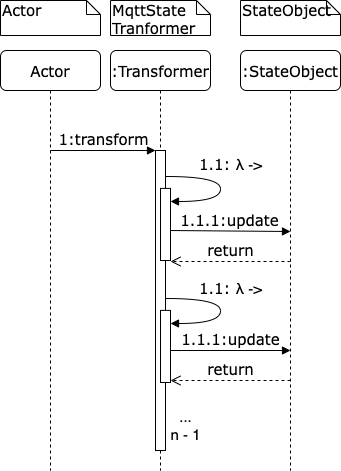
\includegraphics[width=10cm,height=7cm,keepaspectratio]{images/Transformation_old.png}
        \caption{Transformation über Switch-Case-Anweisung}
        \label{fig:sequenceTransformationOld}
    \end{figure}

\begin{lstlisting}[language=Java, frame=lines, xleftmargin=\parindent, style=algoBericht, label={code:switch-case}, captionpos=b, caption={Transformeation über Switch-Case-Anweisung}]
public class MqttTransformer extends AbstractTransformer<InnovationLabKA> {
    private final LogicHubState<InnovationLabKA> logicHubState;
    ...

    public void transform(String topic, String payload) {
        switch (topic) {
            case "InnovationLab/LogicHub/PersonOnDoor":
                logicHubState.setState((innovationLab) -> {
                    innovationLab.setPersonOnDoor(payload);
                    innovationLab.update();
                });
                break;
            case "InnovationLab/LogicHub/SR/GoTo":
                logicHubState.setState((innovationLab) -> {
                    innovationLab.setSRGoTo(payload);
                    innovationLab.update();
                });
                break;
            ... 
        }    
    }
}
\end{lstlisting}
    Dieser Ansatz gibt eine Übersicht des Topics und der dafür vorgesehenen Zustandsänderung. Nachteile dabei sind jedoch, dass die Anweisungen 
    zunehmen, je mehr Regeln und dafür vorgesehen Zustandsänderungen hinzugefügt werden und die einmalige Verwendung der \acs{MQTT}-Topic-Zeichenkette. Dafür muss der 
    Anwender, um innerhalb einer Regel eine weitere Zustandsänderung vornehmen zu können, das Topic erneut aufgreifen und in Kenntnis des jeweiligen sein. Mit dem 
    Topic würde dann über den \acs{MQTT}-Producer eine Nachricht veröffentlicht werden, die die Aktion der Regeländerung steuert. 
    \\
    Diese umständliche Art und Weise galt es dem Anwender zu erleichtern, deshalb wurde ein zweiter Lösungsweg erarbeitet, der in folgendem Abschnitt 
    aufgezeigt wird.

    \subsubsection*{Transformationsobjekt mittels eigenem Objekt}
        In Opposition zu der Verwendung einer Switch-Case-Anweisung wird bei diesem Ansatz eine Klasse implementiert, mit der je nach Bedarf 
        weitere Objekte mit unterschiedlichen Werten erzeugt werden kann. Dabei werden in dem Konstrukt der Klasse die jeweiligen Parameter 
        definiert. Das zu erzeugende Objekt wird zur Laufzeit dem Framework übergeben und in einer Liste gespeichert, sodass das System damit arbeiten kann. 
        Die Parameter, die der Entwickler bestimmt, haben folgende Funktion:
        \begin{itemize}
            \item 1. Parameter: Hier wird das Topic übergeben. Der \acs{MQTT}-Subscriber prüft, ob das konsumierte Topic einem in der Liste definierten Topics entspricht.
            \item 2. Parameter: Hier wird der Key definiert. Das über das Topic mitgelieferte JSON-Konstrukt wird auf diesen key überprüft. Dessen Wert für den Zustandsraum relevant. Hierüber wird der Zustand des Objektes transportiert.
            \item 3. Parameter: Hier wird optional eine Liste übergeben, die nur bestimmt Werte für den Key zulässt, eine sogenannte \textit{White-List}.
            \item 4. Parameter: Hier wird der Name des Feldes im Zustandsraum wiedergegeben, sodass mittels Reflection der Wert im Zustandsraum adressiert werden kann.
        \end{itemize}
        Diese Werte bilden die Transformation, die ebenso für die inverse Transformation (siehe Abschnitt \ref{subsec:inverseTransformation}) gilt.
        Der Ablauf dieser kann dem folgenden Sequenzdiagramm entnommen werden:
    \begin{figure}[hbt!]
        \centering
        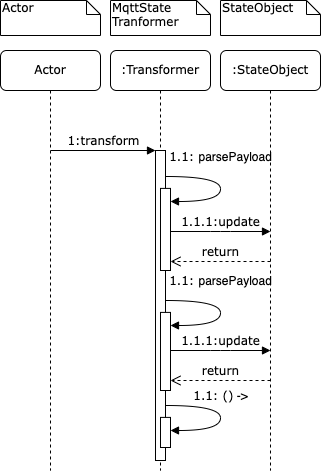
\includegraphics[width=10cm,height=7cm,keepaspectratio]{images/Transformation_new.drawio.png}
        \caption{Transformation über eigenes Objekt}
        \label{fig:sequenceTransformationNew}
    \end{figure}
    \\
    Um das Objekt zu erzeugen, muss der Entwickler lediglich das folgende Code-Beispiel verwenden und auf die entsprechenden Werte anpassen:
\begin{lstlisting}[language=Java, frame=lines, xleftmargin=\parindent, style=algoBericht, label={code:object}, captionpos=b, caption={Transformeation über eigenes Objekt}]
public class InnovationLogicHubApplication {
    public InnovationLogicHubApplication() {
        ... 
        logicHub.addTransformation(
            new SimpleTopicTransformation(
                "InnovationLab/LogicHub/PersonOnDoor",
                "email",
                "personOnDoorEmail"
            )
        );
    }
}
\end{lstlisting}
    Der interne Ablauf des Frameworks unterscheidet sich bei beiden Transformationsmethoden in Nuancen, wie den beiden Sequenzdiagrammen 
    (\ref{fig:sequenceTransformationOld} und \ref{fig:sequenceTransformationNew}) zu entnehmen ist. Jedoch wird bei dem zweiten Ansatz 
    das Zustandsobjekt mittels Reflection manipuliert und anschließend als Änderung registriert und ausgeführt, während bei der ersten Methode 
    die Änderung direkt über die Lambda-Funktion gesteuert und ausgelöst wird. Dies hat für den Anwender keinerlei Auswirkung, relevant hingegen war, 
    welcher Ansatz für den Entwickler den besseren darstellt. An dieser Stelle bringt der zweite Ansatz Potentiale mit, die dem Entwickler die 
    Handhabung der Interaktionen formalisieren und erleichtern und zudem übersichtlicher gestalten.
    \\
    \linebreak
    Für die Vorteile, die der zweite Ansatz dem Entwickler gegenüber bringt, wurde dieser in dem Framework angewendet. 
    \\
    \linebreak
    Die Funktionsweise der Transformation ist demnach wie folgt umgesetzt:
    \\
    Die vorab definierten Transformationen des Entwicklers werden in einer Liste gespeichert, damit das darin enthaltene Topic mit dem eingehenden 
    verglichen werden kann. Dafür wird über die Liste iteriert und jede Transformation, sowie deren zugewiesenes Topic geprüft. Sofern 
    es eine Übereinstimmung gibt, wird der Key-Wert ermittelt und als Nutzlast (\textit{Payload}) übergeben. An dieser Stelle wird der \textit{ReentrantLock} aktiviert 
    und die Feldmanipulation durchgeführt für den Wert, der mittels Nutzlast mitgegeben wurde. Nachdem die Zustandsändeurng erfolgte, wird der \textit{Lock} deaktiviert und 
    die Zustandsänderung an die Logikschicht weitergegeben. Der Ablauf kann dem Sequenzdiagramm (siehe Abbildung \ref{fig:kommunikationsequenz}) entnommen werden. 
    Somit ist die Transformation erfolgt. 
    \\
    Die Funktion der inversen Transformation wird in folgendem Abschnitt erläutert.

\subsection{Inverse Transformation}
\label{subsec:inverseTransformation}
    Damit der Anwender des Frameworks bei der Regeldefinition einen geringen Aufwand erfährt und dennoch dadurch eine weitere 
    Zustandsänderung hervorrufen kann, findet an dieser Stelle eine inverse Transformation stattfinden. Dadurch wird anhand 
    der Zustandsänderung, die der Entwickler durch eine Funktion vorgibt, die zugehörige Aktion mittels \acs{MQTT}-Nachricht 
    veröffentlicht. In Folge dessen muss der Entwickler bei der Implementierung einer Regel keine Kenntnis über das 
    \acs{MQTT}-Topic haben, lediglich muss das richtige Attribut im Zustandsraum angesprochen und geändert werden. 
    Ein konkretes Beispiel: 
    \\
    \linebreak
    Wird ein Lichtschalter eingeschaltet, so wird ein \acs{MQTT}-Topic konsumiert, dass den Zustandsraum ändert, indem 
    der Schalter betätigt wurde. Daraufhin wird eine Regel ausgeführt, deren Regelaktion die LED-Leuchte aktiviert. 
    Dementsprechend definiert der Entwickler eine Funktion, die den Wert des Lichtzustandes im Zustandsobjekt verändert. 
    Mit der Veränderung wird überprüft, um welches Attribut es sich im Zustandsraum handelt und wie sich der Wert geändert hat. 
    Wenn diese Überprüfung zutrifft, wird im Rahmen der inversen Transformation ein \textit{JSON}-Konstrukt generiert, welches 
    mit dem in der Transformation definierten Topic als \acs{MQTT}-Nachricht an den \acs{MQTT}-Broker publiziert wird. 
    Daraufhin wird die LED-Leuchte angeschaltet. 
    \\
    \linebreak
    Zusammengefasst wird mit der inversen Transformation vermieden, dass der Entwickler sich neben der zu definierenden 
    Zustandsänderung zusätzlich um das veröffentlichen der jeweiligen Nachricht und das Verpacken in eine übertragbare 
    \textit{JSON}-Struktur kümmern muss. Des weiteren ist die Kenntnis über das Topics, unter dem die Nachricht 
    gesendet wird, ausschließlich in der Transformation von Nöten und muss nicht an mehreren Stellen konkret 
    aufgeschrieben werden. Hierbei wird dieser Schritt zentralisiert in dem Transformationsobjekt festgehalten. 
%
%Hierfür muss erneut eine  \acs{MQTT}-Nachricht 
%über ein bestimmtes Topic veröffentlicht werden. Diese Veröffentlichung findet im Rahmen der inversen Transformation statt Da diese Transformation bereits definiert wurde, ist innerhalb der Regel %ausschließlich die Zustandsänderung 
%zu definieren. Mithilfe der inversen Transformation wird anhand der Zustandsänderung die dementsprechende Aktion invertiert und unter 
%dem dafür vorgesehenen Topic eine Nachricht veröffentlicht, die die LED konsumiert und daraufhin das Licht angeschaltet. 

\subsection{Zustandsraum}
%Aggregation von Objekten -> Nein
%Aggregation über Serialisierung 
%Objekte können nur einzeln erstellt werden (Einzelner Eintrag oder Objekt mit wiederum einträgen)
% Vermeidung von Rückkopplung 

\subsection{Implementierung eines Anwendungsfalls}
%Erläuterung der Umsetzung des Anwendungsfalls (Mögliche Regeldefinition)
%-> Einbauen von Thread.sleeps um einen durchehenden Prozess zu durchlaufen oder 
% feingranulare Regeln, die immer wieder auf Rückmeldung über MQTT Topics warten und danach die Aktion auslösen


%\subsection{Aufbau der Architektur}
%\subsection{Einbindung der Funktionen abgeleitet von der Konzeption}
\section{Fazit der prototypischen Implementierung}
\subsection{Modellierungsmöglichkeiten}

%Grenzen 
%Modellierungsempfehlungen - Regel, Bedingung und Zustandraum 
%Worauf man achten soll, wenn man ein neues Szenario abbildet. 
%Modellierungsmöglichkeiten des Frameworks.